\documentclass[12pt]{article}
\usepackage[T1]{fontenc}
\usepackage[utf8]{inputenc}
\usepackage{polski}
\usepackage{minted}
\usepackage{geometry}
\usepackage{natbib}
\usepackage{graphicx}
\usepackage{bold-extra}
\usepackage[font=small,labelfont=bf]{caption}
\usepackage{hyperref}
\usepackage{titlesec}
\titlelabel{\thetitle.\quad}

 \geometry{
     left=23mm,
     top=25mm,
     right=23mm
 }


\def\mydate{\leavevmode\hbox{\twodigits\day.\twodigits\month.\the\year}}
\def\twodigits#1{\ifnum#1<10 0\fi\the#1}

\begin{document}
%titlepage
\thispagestyle{empty}
\begin{center}
\begin{minipage}{0.75\linewidth}
    \centering
    
\includegraphics[width=0.45\linewidth]{agh_logo2.png}
    \par
    \vspace{2cm}
    {\bfseries{\scshape{\Huge  Teoria współbieżności}}}
    \par
    \vspace{2cm}
    {\scshape{\Large Laboratorium 1}}
    \par
    \vspace{0.4cm}
    {\scshape{\Large Współbieżność w Javie}}
    \par
    \vspace{3cm}

    {\scshape{\Large Albert Gierlach}}\par
    \vspace{1cm}

    {\Large \mydate}
\end{minipage}
\end{center}
\clearpage



\section{Zadanie 1 oraz 2}
\begin{enumerate}
    \item Napisać program (szkielet), który uruchamia 2 wątki, z których jeden zwiększa wartość zmiennej całkowitej o 1, drugi wątek zmniejsza wartość o 1. Zakładając że na początku wartość zmiennej Counter była 0, chcielibyśmy wiedzieć jaka będzie wartość tej zmiennej po wykonaniu 100000 operacji zwiększania i zmniejszania przez obydwa wątki.
    \item Na podstawie 100 wykonań programu z p.1, stworzyć histogram końcowych wartości zmiennej Counter.
\end{enumerate}
  
\section{Koncept rozwiązania}
Korzystając ze szkieletu aplikacji zaimplementowałem powyższe polecenia, następnie przy pomocy języka Python wygenerowałem histogram wartości zmiennej counter.

\section{Implementacja oraz wyniki}
Dla uproszczenia pominąłem gotową implementację klasy Counter oraz importy.

\begin{minted}[frame=lines,
                framesep=2mm
                ]{java}
class IThread extends Thread {
    public final Counter counter;

    IThread(Counter c) {
        this.counter = c;
    }

    public void run() {
        IntStream.range(0, 100000).forEach(i -> {
            counter.inc();
        });
    }
}

class DThread extends Thread {
    public final Counter counter;

    DThread(Counter c) {
        this.counter = c;
    }

    public void run() {
        IntStream.range(0, 100000).forEach(i -> {
            counter.dec();
        });
    }
}


class Race {
    public static void main(String[] args) throws InterruptedException {
        var results = new ArrayList<Integer>();
        for (int i = 0; i < 100; i++) {
            Counter cnt = new Counter(0);
            var ti = new IThread(cnt);
            var td = new DThread(cnt);

            ti.start();
            td.start();

            ti.join();
            td.join();

            results.add(cnt.value());
        }

        System.out.println(Arrays.toString(results.toArray()));
        saveToFile("./hist1.txt", results);
    }
\end{minted}

Wyniki uruchomienia programu:
\begin{minted}[breaklines]{java}
[-5469, -44562, -12314, 0, 0, 97, 0, 0, 0, 166, -6, 0, 0, 0, -7, 0, 0, 0, 0, -99060, 0, 0, 0, 0, 0, 0, 0, 0, 0, 95887, 0, 0, 0, 0, 0, 0, 0, 0, 0, 94560, 0, 0, 0, 0, 0, 0, 0, 0, 0, 0, 0, 0, 0, 0, 0, 0, 0, 0, 0, 0, 0, 0, 0, 0, 0, 100000, 0, 0, 0, 0, 0, 0, 0, 0, 0, 0, 0, 0, -42351, 0, 0, 0, 0, 0, 0, 61488, 0, 0, 0, 0, 0, 0, 0, 0, 0, 0, 0, 0, 0, 100000]
\end{minted}

\begin{center}
\centering
    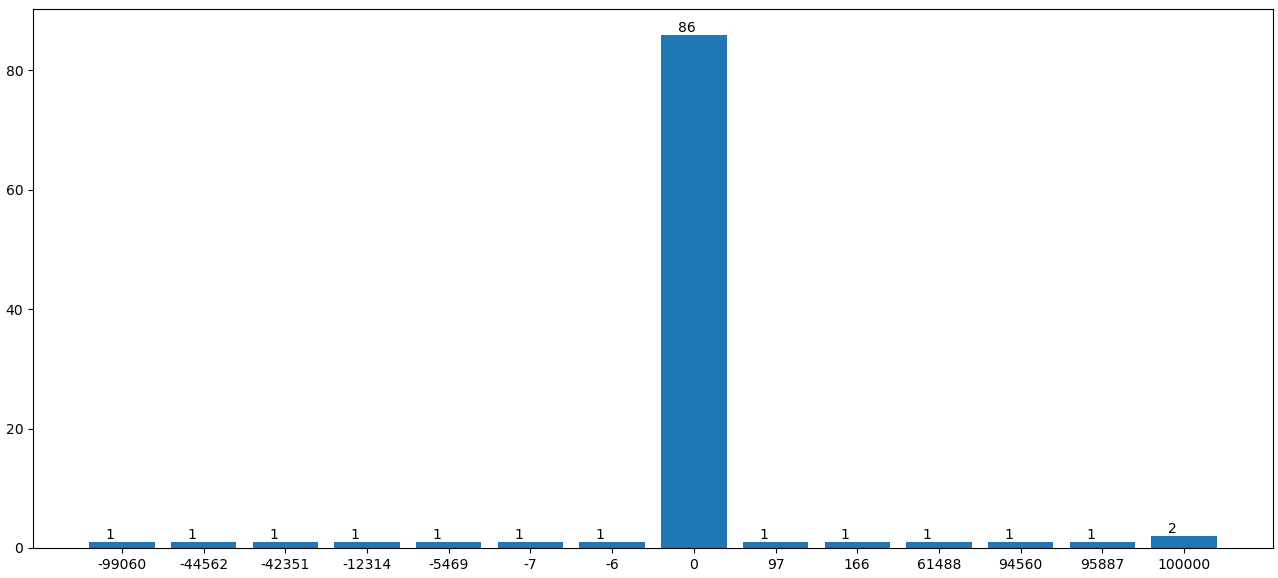
\includegraphics[width=\textwidth]{hist1.png}
    \captionof{figure}{Histogram wartości licznika po wykonaniu operacji}
\end{center}


Jak można zauważyć - większość wartości jest równa zero. Jest to całkowicie niezgodne z przewidywaniami. Po długiej analizie oraz szukaniu informacji w internecie udało się namierzyć źródło problemu. Problemem w tym zadaniu okazały się być optymalizacje, które Java wykonuje, a konkretniej JIT (ang. Just In Time Compiler). Po znalezieniu probemu dodałem do maszyny wirtualnej Javy następujące opcje, które wyłączają JIT:

\begin{minted}{text}
    -Xint -Djava.compiler=NONE
\end{minted}
oraz uruchomiłem ponownie program. Oto otrzymane rezultaty:

\begin{minted}[breaklines]{java}
[-16197, 38, -2234, -2070, 10377, -7944, -4781, 13360, 3757, -23623, 4447, 21242, 15325, -7985, -15077, 5386, 2705, 18416, 5467, -12634, 9760, -1940, -6913, 2208, -237, 946, 1966, 3815, 1440, -266, -1101, -8811, -5997, -1787, -8793, 5782, 2472, -4138, 24127, 3642, -3358, 7144, 18603, 8040, -6988, 10591, 662, -3159, 15307, -6955, 10354, 4185, 6391, 1499, -4352, 2679, 8721, 2989, -6411, -2442, 4185, -7126, 1171, 1105, -1962, 5858, 1984, 2285, -604, -3746, 454, -1853, 2158, 8052, -8676, 220, 42097, 10518, -2104, 22706, 12162, 15850, 9510, -3581, -32393, 2251, 2240, -3924, -7471, -15346, 8026, 343, 3418, 7703, 3947, 2325, -1417, -9413, 11956, 2397]
\end{minted}
Histogram wartości nie został wygenerowany, gdyż każda z wartości występuje raz lub są nieznaczne zwielokrotnienia.

\newpage
\section{Wnioski}
Przeprowadzone testy pokazały, że stosując wątki, które współdzielą dostęp do określonego zasobu, a dostęp ten nie jest synchronizowany, nie mamy żadnej gwarancji, że obliczenia zostaną wykonane poprawnie. Wyniki są całkowicie niedeterministyczne, ponieważ dochodzi do sytuacji wyścigu. Rozwiązaniem takiego dostępu może być zastosowanie mechanizmu synchronizacji jak słówko kluczowe 'synchronized', obiekty typu Atomic lub obiekty typu Semaphore, Lock.


\section{Zadanie 3}
\begin{enumerate}
    \item Spróbować wprowadzić mechanizm do programu z p.1, który zagwarantowałby przewidywalną końcową wartość zmiennej Counter. Nie używać żadnych systemowych mechanizmów, tylko swój autorski.
\end{enumerate}

\section{Koncept rozwiązania}
Pierwszym pomysłem było zaimplementowanie algorytmu Dekkera\footnote{\url{https://en.wikipedia.org/wiki/Dekker\%27s\_algorithm}}, jednak po implementacji okazało się, że dla tak wielu iteracji (100000) jest on zbyt wolny. Wątki spędzają zbyt dużo czasu na oczekiwaniu na dostęp i przekazywaniu sobie dostępu do zasobu. Z racji tego, iż w implementacji nie można było użyć gotowych mechanizmów stwierdziłem, że zaimplementują bardzo prymitywnego zarządcę (scheduler). Będzie to dużo wydajniejsze rozwiązanie, gdyż wątki będą otrzymywać dostęp na określony czas, co pozwoli znacznie przyspieszyć wykonanie operacji. Synchronizacja polega na usypianiu i wybudzaniu wątków za pomocą metod sleep() oraz interrupt(). Zarządca iteruje po wątkach dopóki wszystkie nie zostaną wykonane. 

\newpage
\section{Implementacja oraz wyniki}
Dla czytelności zamieszczam tylko te fragmenty kodu, które są istotne dla tego zadania.
\begin{minted}[frame=lines,
                framesep=2mm
                ]{java}
class MyThread extends Thread{
    public final Counter counter;
    protected final Executor executor;
    private boolean isStarted = false;
    private boolean isFinished = false;
    protected int sleepingTime = 0;

    MyThread(Executor e, Counter c) {
        this.counter = c;
        this.executor = e;
    }

    public void sleep(int time) {
        this.sleepingTime = time;
    }

    public void wakeup(){
        this.sleepingTime = 0;
    }
}

class IThread extends MyThread {
    IThread(Executor e, Counter c) {
        super(e, c);
    }

    public void run() {
        IntStream.range(0, 100000).forEach(i -> {
            if (this.sleepingTime > 0) {
                try {
                    Thread.sleep(this.sleepingTime);
                } catch (InterruptedException e) {
                    this.wakeup();
                }
            }

            counter.inc();
        });
        this.executor.notifyAboutFinished(this);
    }
}

class DThread extends MyThread {
    DThread(Executor e, Counter c) {
        super(e, c);
    }

    public void run() {
        IntStream.range(0, 100000).forEach(i -> {
            if (this.sleepingTime > 0) {
                try {
                    Thread.sleep(this.sleepingTime);
                } catch (InterruptedException e) {
                    this.wakeup();
                }
            }

            counter.dec();
        });
        this.executor.notifyAboutFinished(this);
    }
}

class Executor{
    private final List<MyThread> threads;
    private int finishedNum = 0;
    private final int SWITCH_TIME = 10;

    public Executor(){
        threads = new ArrayList<>();
    }

    public void addThread(MyThread t){
        threads.add(t);
    }

    public void delay(int time){
        try {
            Thread.sleep(time);
        } catch (InterruptedException e) {
            e.printStackTrace();
        }
    }

    public void start(){
        do {
            finishedNum = 0;
            threads.forEach(current -> {
                if (current.isFinished()) {
                    finishedNum++;
                    return;
                }

                if (current.isStarted()) {
                    current.interrupt(); // wake up thread
                } else {
                    current.setStarted(true);
                    current.start(); // start thread
                }

                delay(SWITCH_TIME); // give time for thread to operate
                current.sleep(SWITCH_TIME * threads.size() * 3); //suspend scheduler
                delay(SWITCH_TIME); //give time for thread to sleep
            });

        } while (finishedNum != threads.size());

        threads.forEach(t ->{ //let threads finish/close
            try{
                t.join();
            }catch (Exception ignored){}
        });
    }

    public void notifyAboutFinished(MyThread thread){
        thread.setFinished(true);
        this.finishedNum++;
    }
}

class Race {
    public static void main(String[] args) {
        var results = new ArrayList<Integer>();

        for (int i = 0; i < 100; i++) {
            Executor e = new Executor();
            Counter cnt = new Counter(0);
            e.addThread(new IThread(e, cnt));
            e.addThread(new DThread(e, cnt));

            e.start();

            results.add(cnt.value());
        }

        System.out.println(Arrays.toString(results.toArray()));
        var res = results.stream().allMatch(i -> i == 0);
        System.out.println("All elements are zero? " + res);
    }
}
\end{minted}

\begin{minted}[breaklines]{java}
[0, 0, 0, 0, 0, 0, 0, 0, 0, 0, 0, 0, 0, 0, 0, 0, 0, 0, 0, 0, 0, 0, 0, 0, 0, 0, 0, 0, 0, 0, 0, 0, 0, 0, 0, 0, 0, 0, 0, 0, 0, 0, 0, 0, 0, 0, 0, 0, 0, 0, 0, 0, 0, 0, 0, 0, 0, 0, 0, 0, 0, 0, 0, 0, 0, 0, 0, 0, 0, 0, 0, 0, 0, 0, 0, 0, 0, 0, 0, 0, 0, 0, 0, 0, 0, 0, 0, 0, 0, 0, 0, 0, 0, 0, 0, 0, 0, 0, 0, 0]
All elements are zero? true
\end{minted}

\section{Wnioski}
Pomimo, iż powyższy zarządca jest zaimplementowany bardzo naiwnie, to udało się zagwarantować przewidywalne wyniki. Program działa stosunkowo szybko, z uwagi na to, że każdy wątek otrzymuje swój kwant czasu, który wykorzystuje na obliczenia, co znacznie przyspiesza wykonanie. Warto dodać, że powyższy scheduler wspiera zarządzanie więcej niż dwoma wątkami.

\section{Zadanie dodatkowe}
W systemie dziala N wątkow, które dzielą obiekt licznika (początkowy stan licznika = 0).

Każdy wątek wykonuje w pętli 5 razy inkrementację licznika. Zakładamy, że inkrementacja składa się z sekwencji trzech instrukcji: read, inc, write (odczyt z pamięci, zwiększenie o 1, zapis do pamięci). Wątki nie są synchronizowane.
\begin{enumerate}
    \item Jaka jest teoretycznie najmniejsza wartość licznika po zakończeniu działania wszystkich wątków i jaka kolejność instrukcji (przeplot) do niej prowadzi?
    \item Spróbować znaleźć dowód, że będzie to zawsze najmniejsza wartość.
\end{enumerate}

\section{Koncept i rozwiązanie}
W rozwiązaniu trzeba oczywiście skorzystać z sytuacji, w której dochodzi do wyścigu. Idea polega na tym, aby jeden z wątków nadpisał wyniki obliczeń N-2 wątków, a jeszcze kolejny skorzystał z wartości obliczonej przez wcześniej wspomniany wątek. W efekcie czego wartość licznika zostanie nadpisana i będzie równa 2. Jest to możliwe dzięki temu, że operacja zwiększenia licznika nie jest atomowa (ponieważ składa się z 3 osobnych instrukcji)
\par
Sekwencja, która prowadzi do takiego wyniku może wyglądać następująco:
\begin{itemize}
    \item Wybierzmy dwa wątki spośród N i oznaczmy je literami A oraz B
    \item Wątek A odczytuje wartość licznika (zero) oraz inkrementuje ją, ale jeszcze nie zapisuje
    \item Pozostałe N-2 wątków wykonuje się aż do zakończenia swoich operacji
    \item Wątek B wykonuje 4 z 5 iteracji
    \item Wątek A zapisuje wartosć 1 do licznika
    \item Wątek B rozpoczyna swoją ostatnią iterację - wczytuje wartość 1 oraz inkrementuje ją
    \item Wątek A wykonuje pozostałe 4 iteracje
    \item Wątek B zapisuje wartość 2 w liczniku
\end{itemize}

Powyższą sekwencję, można wykonać dla dowolnej ilości wątków większej niż jeden, ponieważ wystarczą nam dwa wątki, aby móc zmanipulować wykonanie w taki sposób, aby wspomniane wątki nadpisały swoją zawartość.


\end{document}
